%! Author = adnansiddiquei
%! Date = 08/03/2024

\section{Selection of Solution Algorithm and Prototyping}\label{sec:prototyping}
    \begin{figure}[htb]
    \centering
    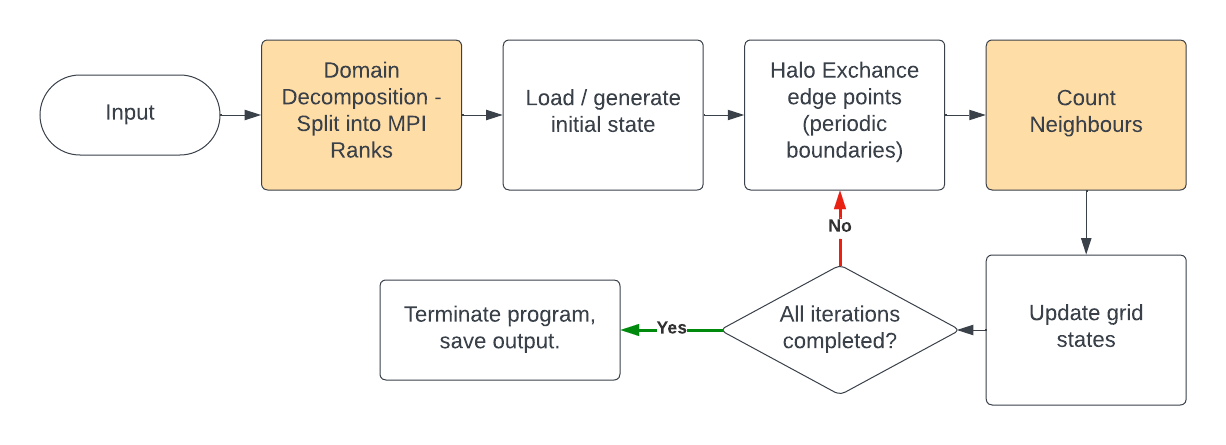
\includegraphics[width=0.9\textwidth]{./figures/high-level-flowchart}
    \caption{A high-level flow chart depicting the algorithm. The key points for efficiency considerations
    are highlighted in red, the considerations are discussed in the main text.}
    \label{fig:high-level-flowchart}
    \end{figure}

    Fig.\eqref{fig:high-level-flowchart} shows the high-level algorithm being used to simulate Conway's
    Game of Life.
    The key points of consideration with regard to performance are highlighted in red.
    There are 3 domain decomposition methods available (column, row and block decomposition) as well as multiple
    ways to count neighbours and update grid states.
    As indicated in Fig.\eqref{fig:high-level-flowchart}, communication overheads between MPI ranks can be hidden
    behind computation by using non-blocking communication and counting whichever neighbours are available at the time.
    Likewise, the actual method of counting neighbours and updating the grid can be done in a variety of ways, each with
    their own merits.
    All these considerations are discussed thoroughly in this section, and then they are investigated in the next
    section.

    \subsection{Domain Decomposition and Neighbour Counting Algorithm}\label{subsec:domain-decomp}
    Domain decomposition can be done by either strips or blocks.
    Strips has the advantage that it is simpler to implement but will have more memory needing to be passed between
    boundaries, with the opposite being true for blocks.
    Therefore, the choice of domain decomposition will need to be tested to see which is more efficient as the data
    size and number of MPI ranks increases.
    However, the overheads of communication can be effectively nullified if the communication is hidden behind computation,
    as such, this also needs to be explored to see what proportion of the communication can be hidden.

    The neighbour counting algorithm has 2 possible implementations, a simple convolution and a separable kernel.
    \begin{itemize}
        \item \textbf{Simple convolution.} Loop through each cell, and count the number of neighbours.
            This is equivalent to a 3x3 convolution with the below kernel.
            \begin{equation}
            \begin{bmatrix}
            1 & 1 & 1 \\
            1 & 0 & 1 \\
            1 & 1 & 1 \\
            \end{bmatrix}\label{eq:kernel1}
            \end{equation}
            This requires a total of $8N^{2}$ addition operations (the $9N^{2}$ multiplication operations that would usually occur can
            be ignored because the kernel only contain 1s and 0s so we can skip the multiplication operation in this special case).
        \item \textbf{Separable kernel.} If the following kernel is used instead,
            \begin{equation}
            \begin{bmatrix}
            1 & 1 & 1 \\
            1 & 1 & 1 \\
            1 & 1 & 1 \\
            \end{bmatrix}\label{eq:kernel2}
            \end{equation}
            then the kernel becomes separable.
            This means that the kernel can be split into two 1D identical kernels \(\begin{bmatrix} 1 & 1 & 1 \end{bmatrix}\) and
            applied in two passes which yields $2N^{2}$ addition operations per pass, yielding a total of $4N^{2}$ operations \cite{separable-kernel}.
            After another ${N^{2}}$ addition operations, to correct for replacing the central 0 with a 1, the total number of
            operations becomes $5N^{2}$.
            Therefore, the separable kernel method yields a theoretical speedup of $8/5 \approx 1.6$.
            However, due to strided memory access on the vertical pass, the speedup will be less than this.
            Although, the vertical pass can be made more efficient by transposing the grid and making the data contiguous,
            it will need to be investigated whether the additional overhead of transposing the grid yields any speedup.
    \end{itemize}

    The simple convolution method would prefer column-wise decomposition as it would reduce the number of cache misses
    when counting the 6 neighbours that are not horizontally adjacent to the current cell.
    This is because shorter rows would reduce the distance in memory between a cell and it's vertical neighbour.
    Theoretically, the separable kernel should not have this issue if the separable convolution can be applied in two horizontal
    passes with a transpose in between.

    \subsection{Hiding Communication Behind Computation}\label{subsec:hiding-comms}
    To the extent of hiding communication behind computation, the separable convolution allows naturally for the horizontal
    pass to be done first, and then the vertical pass to be done after the vertical halos have been exchanged.
    Doing the vertical pass first is also possible but likely to be less efficient due to the strided memory access.
    This would, however, only hide communication if the horizontal halos arrive before the vertical halos which is not guaranteed.
    Given that the horizontal halo exchange involves the exchange of non-contiguous data (assuming the grid is represented
    as a 1D array in row-major order), unless the horizontal halos are smaller than the vertical halos (which would be
    the case in row decomposition), the communication will likely not be hidden behind computation.
    There are other factors such as physical positioning of the MPI ranks and the network topology that will also affect
    the communication overheads between MPI ranks, so it is hard to predict how much time could be consistently saved by
    hiding communication in this method.

    The alternative option for hiding communication is to count the neighbours with the simple convolution
    for all the cells that are not on the boundary, and then count the neighbours for the cells on the boundary once the halo
    exchange has been completed (note, this method is later referred back to as the 'SimpleIO' method).
    The downside of this is that it involves a lot of non-contiguous memory access, which is not ideal for performance, but
    how this method compares to the previous method as the simulation scaled will need to be investigated.

    \subsection{Updating Grid}\label{subsec:update-grid}
    Given the neighbour count and the current state of the grid, there are a few possible ways to update the grid \cite{branchless-programming}.
    \begin{itemize}
        \item \textbf{\inlinecode{if} statements.} This is the most straightforward implementation.
        The minimum number of \inlinecode{if} statements required to implement the rules of Conway's Game of Life is 3,
        and it is unlikely the CPU will be able to optimise this to any degree with branch prediction, so
        this method will likely be the slowest.
        \item \textbf{Bitwise operations.} This method removes all \inlinecode{if} statements and replaces them with
            inline bitwise (\inlinecode{&&} and \inlinecode{||}) operations.
        \item \textbf{Lookup table.} Given that there is only 18 states a cell can be in (dead or alive, with 0 to 8 neighbours),
            a lookup array can be used to update the grid with the new state of each cell, given one of the current
            18 states.
    \end{itemize}
    The efficacy of these methods will need to be tested to see which is the most efficient.

    \subsection{OpenMP with MPI}\label{subsec:omp-with-mpi}
    The final consideration is to assess how to use OpenMP with MPI.
    Not all loops will be infinitely parallelisable, more threads won't always yield a linear speedup.
    Likewise, more MPI ranks yields more communication overheads, and as such there will be trade-offs in this respect.
    The trade-off between OpenMP and MPI will need to be investigated empirically to see what the best combination is.



